\documentclass[../main.tex]{subfiles}
\begin{document}
\subsubsection{Results}\label{subsubsec:results_tanh_shift}

\begin{figure}[H]
    \centering 
    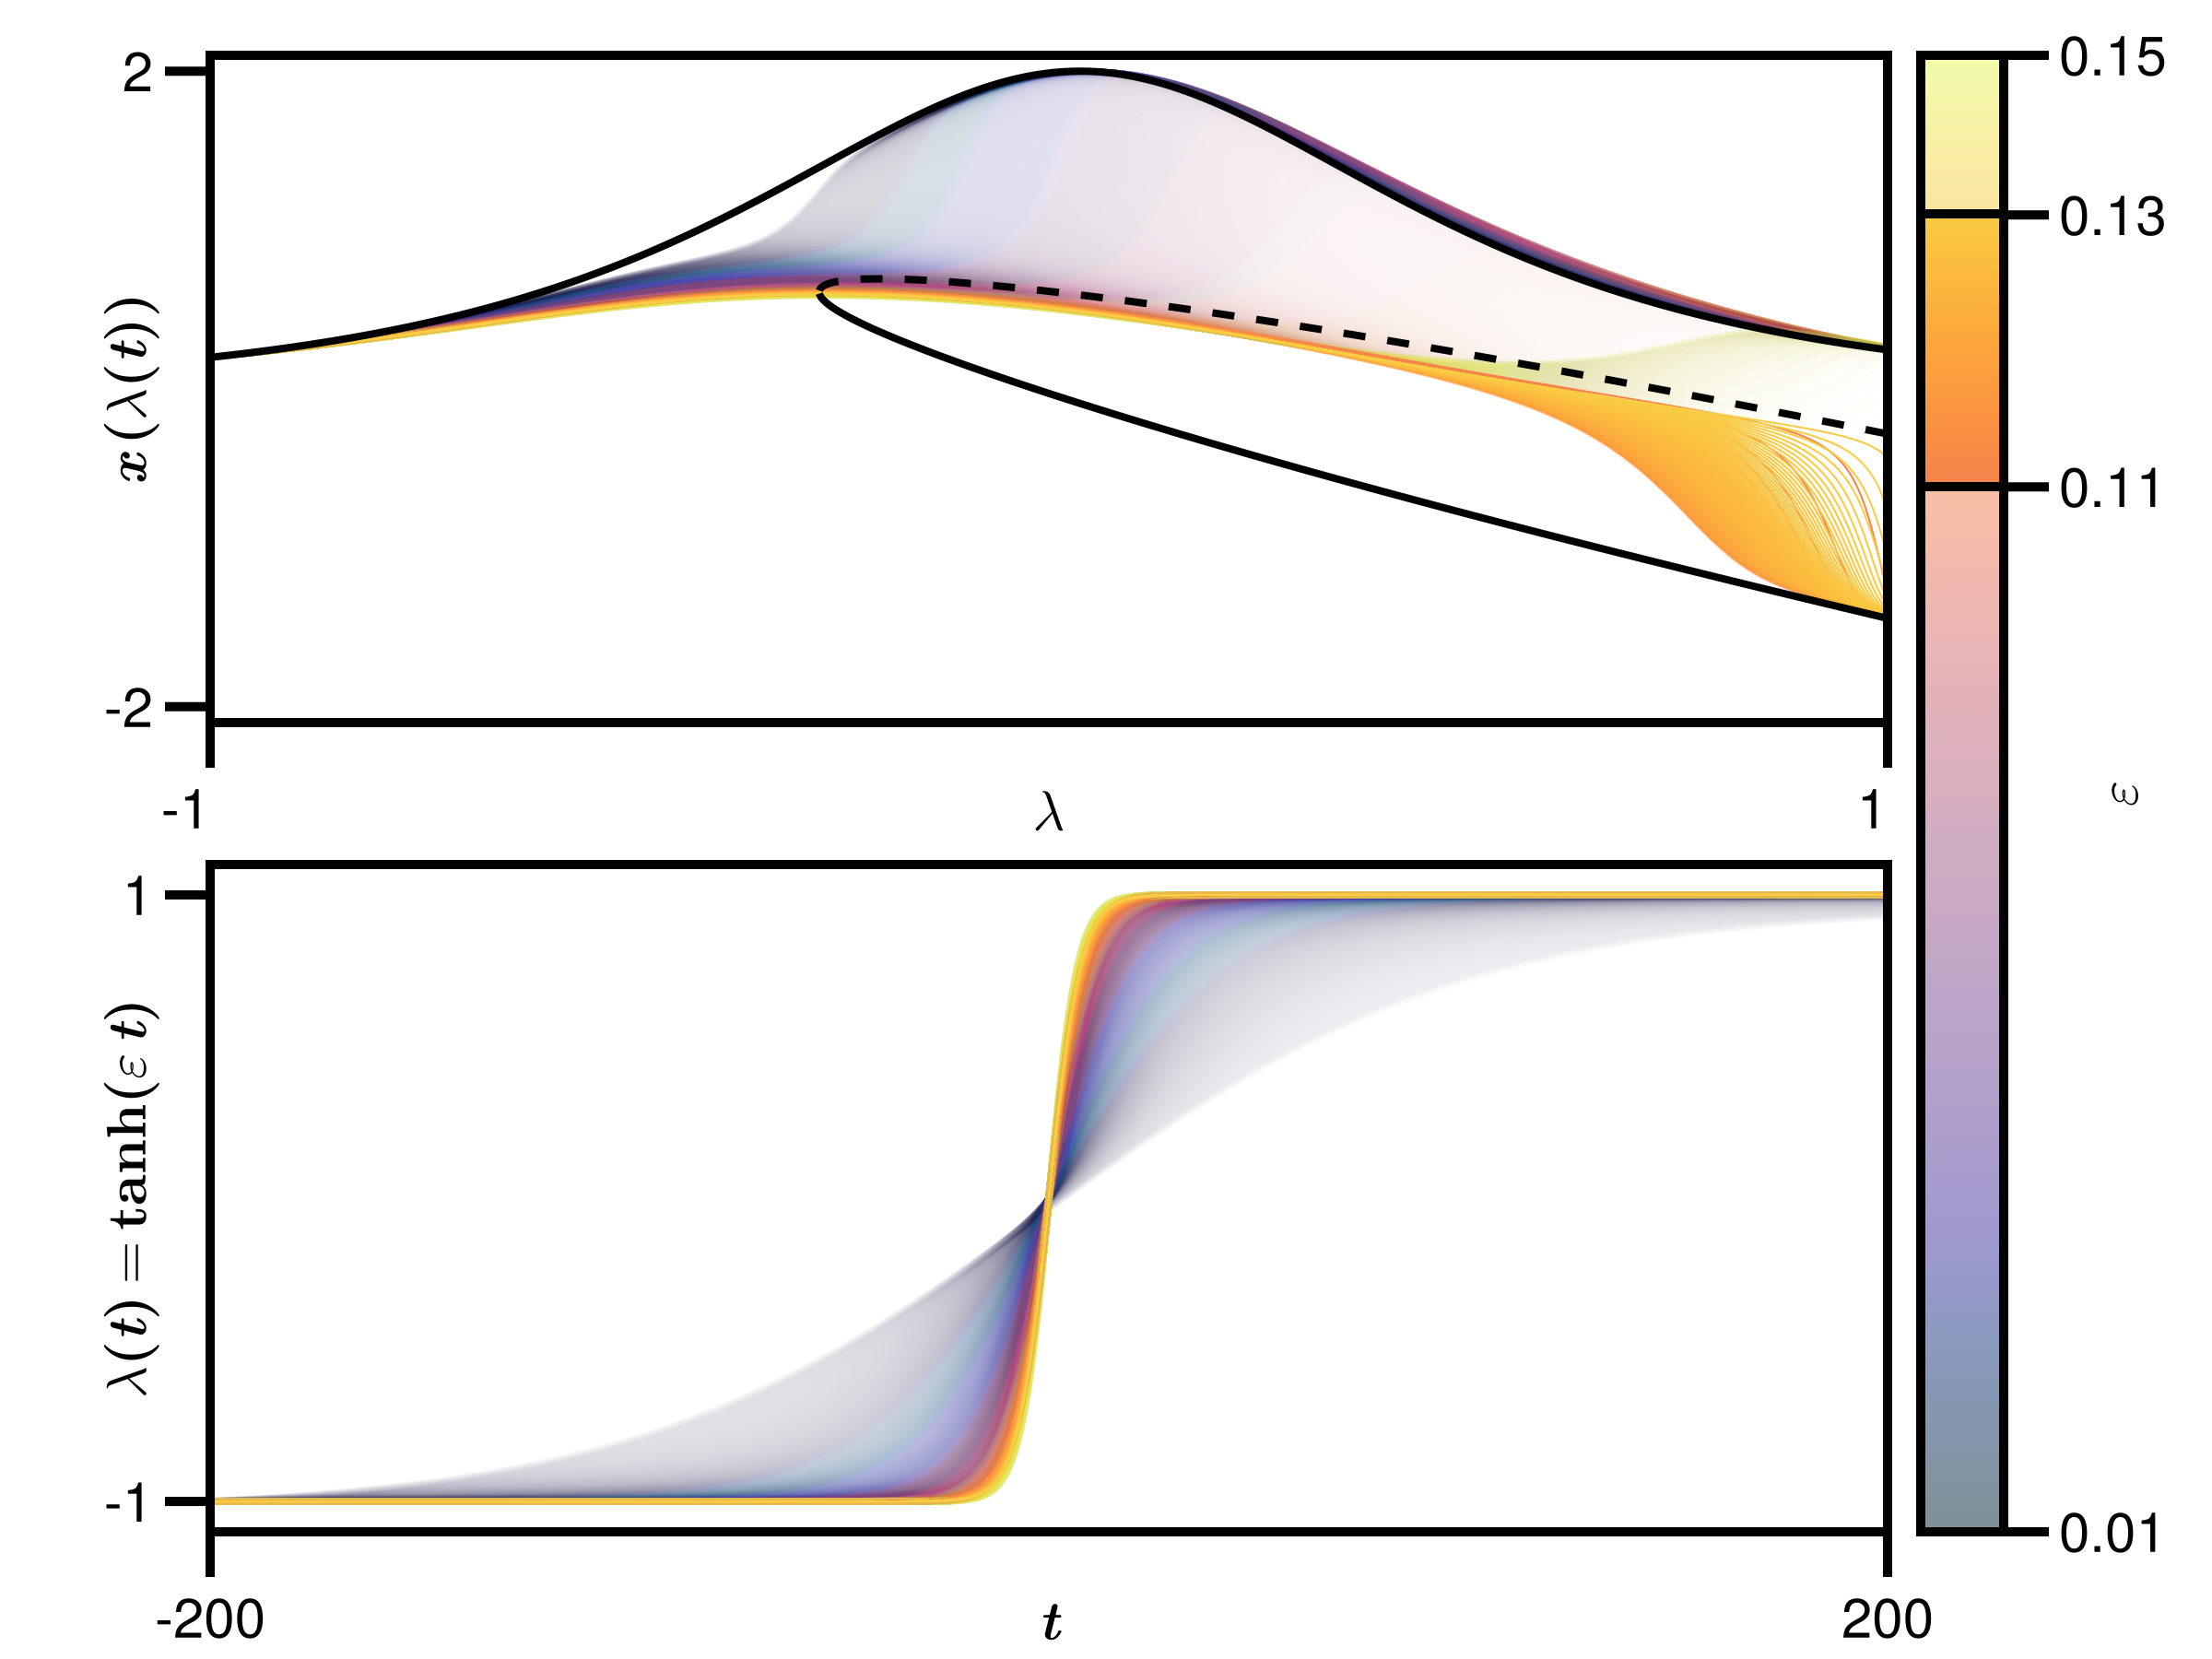
\includegraphics[keepaspectratio, width=\textwidth]{../figures/rate_sweep.png}
    \caption{Family of solutions of \eqref{eq:dyn_sys} with parameter shift \eqref{eq:tanh_shift} for different values of rate $\varepsilon\in[0.01,0.15]$. 
    The range of values for which the solution undergoes irreversible R-tipping (critical tange) is highlighted in the colorbar and roughly corresponds to the set [0.11,0.13].}
    \label{fig:rate_sweep}
\end{figure}


\end{document}
